\subsubsection{Introduction}\label{introduction}

Building systems that depends on \textbf{availability},
\textbf{reliability}, \textbf{safety}, \textbf{maintainability}.\\
A \textbf{failure} is the result of an \emph{error}, that is a caused by
a \emph{fault}.\\
A system is said to be \textbf{fault tolerance} if it can provide its
services even in the presence of faults.\\
Faults are of three types:
\begin{itemize}
\itemsep1pt\parskip0pt\parsep0pt
\item
  \emph{Transient faults}: faults which occur once and disappear
\item
  \emph{Intermitted faults}: faults which appear and disappear with no
  apparent reason (worst faults)
\item
  \emph{Permanent faults}: faults which continue to exist until the
  failed components are repaired
\end{itemize}
Failures are of three types:

\begin{itemize}
\itemsep1pt\parskip0pt\parsep0pt
\item
  \emph{Omission failures} (e.g.~crash)
\item
  \emph{Timing failures} (e.g.~timeout latency of a channel)
\item
  \emph{Byzantine} (continue executing but something different from you
  expect)
\end{itemize}
\textbf{Redundancy} is best way to solve these problems. We can have several types of redundancy:

\begin{itemize}
\itemsep1pt\parskip0pt\parsep0pt
\item
  \emph{Information redundancy} (e.g.~Hamming codes)
\item
  \emph{Time redundancy} (i.e.~try again)
\item
  \emph{Physical redundancy}
\end{itemize}

Let's take the client-server architecture as an example. In the client-server architecture nobody tells me if the server crashed and
at what point of their procedure is crashed. There are many strategies
useful to bypass this problem and obtaining a result, but it's important
to highlight that never I can guarantee exactly one result, such as in
the \emph{printer client-server example}. All strategies turn out to be
suboptimal, since I can get at most one or at least one result.

When clients crash the computation running on server called by that
clients are said to be \textbf{orphan}. In this case the server can have
several approaches:

\begin{itemize}
\itemsep1pt\parskip0pt\parsep0pt
\item
  \emph{Extermination}: RPC's are logged by the client and orphans
  killed by a client request after a reboot (costly because I have to
  keep all logged and there are also problems with network partitions)
\item
  \emph{Reincarnation}: when a clients reboots it starts a new epoch and
  sends a broadcast message to servers, who kill old computations
  started on behalf of that client
\item
  \emph{Gentle reincarnation}: as before but servers kill old
  computations only if owner cannot be located
\item
  \emph{Expiration}: remote computation expire after some time and so,
  clients wait to reboot to let remote computations expire
\end{itemize}

\begin{center}\rule{3in}{0.4pt}\end{center}

\subsection{Protection against process
failures}\label{protection-against-process-failures}

\subsubsection{Process resilience}\label{process-resilience}

Let us assume a context in which channels are reliable but process are not. In this context \textbf{Redundancy} can be used to mask the presence of faulty
processes, with redundant process groups. In practice, the work that
should be done by a process is taken care by a group of processes, and
so the healthy processes can continue to work when come of others fail.\\
Two possible organizations:

\begin{itemize}
\itemsep1pt\parskip0pt\parsep0pt
\item
  \textit{Flat group}
\item
  \textit{Hierarchical group} with workers and a coordinator
\end{itemize}

However, using groups is not so easy because we must keep track of
processes composing a group and, moreover, having a coordinator seems easier but it's a single point of failure.
Finally, it is important to notice that if too many processes crash or leave, the group has to be rebuilt.\\
When we have a group it's also crucial to understand how large a group has to be:

\begin{itemize}
\itemsep1pt\parskip0pt\parsep0pt
\item
  If processes fail silently, then \emph{k+1} processes allow the system
  to be \emph{k-fault tolerant}
\item
  If failures are Byzantine, we need \emph{2k+1} processes in order to
  achieve \emph{k-fault tolerance} and also have a working voting
  mechanism.
\end{itemize}

\subsubsection{Agreement in a process group}\label{agreement-in-a-process-group}
By \textit{agreement in a process group} we mean the reaching a decision among all non-faulty processes, based on the initial values.\\
In order to reach an \textit{agreement in a process group}, these properties must hold:

\begin{itemize}
\itemsep1pt\parskip0pt\parsep0pt
\item
  \emph{Agreement:} no two processes decide on different values
\item
  \emph{Validity}: if all processes start with the same value, then that
  value is the only possible decision value
\item
  \emph{Termination}: all non-faulty processes eventually decide
\end{itemize}

When the communication channels are not reliable it's not possible to
reach a consensus, but \textit{it's possible when we have communication channels reliable and non-reliable processes.}

\textbf{FloodSet Algorithm}\\
\textit{Procedure}\\
\begin{itemize}
    \item Let $v_0$ be a pre-specified default value
    \item Each process maintains a variable $W$ \textit{(subset of V)} initialized with its start value
    \item For $f+1$ rounds:
    \begin{itemize}
        \item Each process sends $W$ to all other processes
        \item It adds the received sets to $W$
    \end{itemize}
    \item After $f+1$ rounds:
    \begin{itemize}
        \item if $|W| = 1$: decide on $W$'s element, so all processes agree on the same value
        \item if $|W| > 1$: decide on $v_0$ or, in alternative, use a common function to decide \textit{(e.g. $min(W)$)}
    \end{itemize}
\end{itemize}

We notice that with this algorithm, each process needs to know the
entire set \emph{W} only if $|W| > 1$. To improve this algorithm we can broadcast \emph{W} at the first round and we go on only if $|W| > 1$.

\textbf{Agreement in a process group in present of byzantine faults}\\
If we have a process group in which there may be byzantine faults the properties change:

\begin{itemize}
\itemsep1pt\parskip0pt\parsep0pt
\item
  \emph{Agreement:} no two \textbf{non-faulty} processes decide on
  different values
\item
  \emph{Validity}: if all \textbf{non-faulty} processes start with the
  same value, then that value is the only possible decision value
\item
  \emph{Termination}: all non-faulty processes eventually decide
\end{itemize}

This problem can be formalized as the generals problems with traitors.
Lamport (1982) showed that if there are m traitors, $2m+1$ loyal
generals are needed for an agreement to be reached, for a total of
$3m+1$. Moreover, \textit{it's proved that is not possible to reach an agreement if there is one faulty process in an asynchronous system}.

\begin{center}\rule{3in}{0.4pt}\end{center}

\subsection{Reliable group
communication}\label{reliable-group-communication}
Let us assume the following properties:
\begin{itemize}
\itemsep1pt\parskip0pt\parsep0pt
\item
  Groups are fixed
\item
  Processes are non-faulty
\item
  Channel is faulty
\end{itemize}

In order to achieve a \textit{reliable group communication} we can have two strategies:
\begin{itemize}
\itemsep1pt\parskip0pt\parsep0pt
\item
  Positive acknowledgements: we send every time \textit{ACKs} \textit{(Pessimist
  approach)}
\item
  Negative acknowledgements: we send \textit{NACKs} when something goes wrong \textit{(Optimist approach)} 

\end{itemize}

\textbf{Note that,} the second approach has a problem: \textit{how the client know that him has to receive a packet and so send a NACK?}

\subsubsection{Non-faulty processes with faulty
channels}\label{non-faulty-processes-with-faulty-channels}

\paragraph{Scalable reliable multicast}\\
The main \textit{idea} is that if a process discovers that something went wrong, notify the error to the other receivers in the net and then also to the sender.\\
\textit{More in detail, }
when an host discovers that something went wrong, \textit{e.g. it didn't receive a packet}, it notifies the error to all the other receivers with an \textit{NACK} message in such a way to cause the suppression their feedback.\\
Once do that, the host sends a \textit{NACK} to the sender after waiting for the timeout to expire. The timeout is indicated by the letter \textit{T} in the image below and it's set randomly. In this way the sender receives only one \textit{NACK}.\\
Note that, the situation doesn't change if two ore more hosts has the same \textit{random delay} timeout.

\paragraph{Hierarchical feedback control}\label{hierarchical-feedback-control}

The main \textit{idea} is that receivers are organized in groups headed by a coordinator
and groups are organized in a tree routed at the sender.

\textit{More in detail}, the coordinator takes care about its group and it can remove a message
from its buffer if it has received an \textit{ACK} from:

\begin{itemize}
\itemsep1pt\parskip0pt\parsep0pt
\item
  All the receivers in its group
\item
  All of its child coordinators
\end{itemize}

The main \textit{problem} here is that the hierarchy has to be built and maintained.

\subsubsection{Faulty processes with non-faulty
channels}\label{faulty-processes-with-non-faulty-channels}

If we have faulty processes and non-faulty channel, things becomes harder. In this case we have to face with the \emph{atomic multicast problem}, that is, a message must be delivered either to all the members of a group or to none, and that the order of the messages be the same at all receivers.\\
The typical example is the order of command in a database transaction.\\
Ideally we want to achieve \textbf{close synchrony}:

\begin{itemize}
\itemsep1pt\parskip0pt\parsep0pt
\item
  We want that any two processes that receive the same multicast
  messages or observe the same group membership changes to see the
  corresponding events in the same order
\item
  We want that a multicast to a process group is delivered to its full
  membership
\end{itemize}
However, \textit{close synchrony} cannot be achieved in the presence of failures.

\subsubsection{Failure detection}\label{detect-a-failure}
In most of systems, a failure detection mechanism is needed in order to understand if something went wrong during the execution of a procedure. However, it's important to notice that, even if we detect a failure we cannot know whether a failed process has received and processed a message.
With this introducation, the model becomes:
\begin{itemize}
\itemsep1pt\parskip0pt\parsep0pt
\item
  Crashed processes are purged from the group and have to join again
\item
  Messages from a correct process are processed by all correct processes
\item
  Messages from a failing process are procced either by all correct
  members or by none
\item
  Only relevant messages are received in a specific order
\end{itemize}

\subparagraph{Virtual synchrony}
It's a form or reliable multicast in which group view changes are delivered in a consistent order with respect to other multicasts and with respect to each other.\\

In order to better understand what \textit{virtual synchrony} is, let us introduce some definitions:
\begin{itemize}
    \item \textbf{Group view:} set of processes to which a message should be delivered as seen by the sender at sending time
    \item \textbf{View change}: it happens when a process joins or leaves the group, possibly crashing
\end{itemize}

In other words, all multicasts must take place between view changes, so that, a
multicast make sense when it's received before that the "news" that a process crashed arrive.

In practice:
\begin{itemize}
\itemsep1pt\parskip0pt\parsep0pt
\item
  We must guarantee that messages are always delivered before or after a
  view change
\item
  If the view change is the result of the sender of the message \emph{m}
  leaving, the message is either delivered to all group members before
  the view change is announced or it's dropped.
\end{itemize}
Generally speaking, multicasts take place in epochs separated by group memebership changes.

Retaining the virtual synchrony property, we can identify different orderings for the multicast messages. In particular we can have:
\begin{itemize}
    \item Unordered multicasts
    \item FIFO-ordered multicasts
    \item Causally-ordered multicasts
\end{itemize}
In addition, the above orderings can be combined with a \textit{total ordering} requirement, so whatever is the chosen order, messages must be delivered to every group member in the same order. Note that, \textit{virtual synchrony} includes this property in its own definition.\\
Moreover, a virtual synchronous reliable multicast ordering totally-ordered delivery of messages is defined as \textbf{atomic multicast}.

\subparagraph{Implementation}\label{implementation}
Over the years, several implementations of \textit{virtual synchrony} have been proposed, for example the one implemented in \textit{ISIS}, that is a fault tolerant distributed system.

However, the basic idea is composed by few key points:
\begin{itemize}
    \item We assume that processes are notified of view changes
    \item When a process receives a view change message, stop sending new messages until the new view is installed, instead it multicasts all pending unstable messages to the non faulty members of the old view, marks them as stable and multicasts a flush message
    \item Eventually, all the non faulty members of the old view will receive the view change and do the same. Obviously, view changes duplicates are discarded.
    \item Each process installs the new view as soon as it has received a flush message from each other process in the new view.
\end{itemize}
After all these points are met, processes can restart sending new messages.\\
In conclusion, if we assume that the group membership does not change during the execution of the protocol above we have that at the end all non faulty members of the old view receive the same set of messages before installing the new view.

\subparagraph{Example}
\begin{figure}[htbp]
\centering
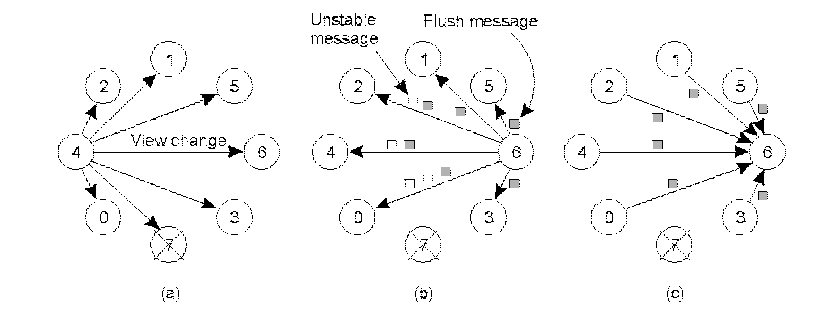
\includegraphics{src/images/fault-tolerance/VS.png}
\caption{An example of view change}
\end{figure}

\begin{enumerate}
    \item Process 4 notices that process 7 has crashed and so it sends a view change
    \item Process 6 sends out all its unstable messages, followed by a flush message
    \item Process 6 installs the new view when it has received a flush message from everyone else
\end{enumerate}

\begin{center}\rule{3in}{0.4pt}\end{center}

\subsection{Distributed commits}\label{distributed-commits}

\textbf{Termination:}

\begin{itemize}
\itemsep1pt\parskip0pt\parsep0pt
\item
  \emph{Weak:} if there are no faults, all processes eventually decide
\item
  \emph{Strong:} all non-faulty processes eventually decide
\end{itemize}

\subsubsection{Two-phase commit}\label{two-phase-commit}

It's a blocking protocol, it satisfies the weak condition and it's allow
to reach termination in less than \emph{f+1} rounds.

\begin{figure}[htbp]
\centering
\includegraphics{C:/Users/Davide/AppData/Roaming/Typora/typora-user-images/image-20200106143546837.png}
\caption{image-20200106143546837}
\end{figure}

If a participant fails, after a timeout a coordinator can assume abort
decision by participant

If the coordinator fails:

\begin{itemize}
\itemsep1pt\parskip0pt\parsep0pt
\item
  If participant blocked waiting for vote request, it can decide to
  abort
\item
  If participant blocked waiting for global decision, it cannot decide
  on its own but it mast wait for the coordinator to recover (blocking
  protocol)
\end{itemize}

\subsubsection{Three-phase commit}\label{three-phase-commit}

It's a non-blocking protocol and it satisfies the strong termination
condition

\begin{figure}[htbp]
\centering
\includegraphics{C:/Users/Davide/AppData/Roaming/Typora/typora-user-images/image-20200106144731846.png}
\caption{image-20200106144731846}
\end{figure}

\begin{figure}[htbp]
\centering
\includegraphics{C:/Users/Davide/AppData/Roaming/Typora/typora-user-images/image-20200106144855466.png}
\caption{image-20200106144855466}
\end{figure}

\begin{center}\rule{3in}{0.4pt}\end{center}

\subsection{Recovery techniques}\label{recovery-techniques}

When processes resume working after a failure, they have to be taken
back to a correct state

There are two types of recovery:

\begin{itemize}
\itemsep1pt\parskip0pt\parsep0pt
\item
  The system is brought back to a previously saved correct state
  (\emph{backward})
\item
  The system is brought into a new correct state from which execution
  can be resumed (\emph{forward})
\end{itemize}

Recovery a previous state is possible only if there is a checkpoint or a
logging system

\subsubsection{Checkpointing}\label{checkpointing}

We need to find a (possibly the most recent) consistent cut. The idea is
going back until we find a couple of checkpoints which give us a
consistent checkpoint, in some kind of domino effect.

One idea is to have an \textbf{independent checkpointing}, where every
process records is own state. However, independent checkpoint is not
trivial to implement, because interval between two checkpoints is tagged
and each message exchanged by the processes must be record a reference
to the interval. It's important to notice that in this way the receiver
can record the dependency between receiving and sending intervals with
the rest of the recovery information.

When a failure occurs, the recovering process broadcast a dependency
request to collect and compute dependency information. All processes
stop and send their information to the recovering process, that computes
the recovery line and sends the corresponding rollback request.

The recovery line can be computed using two different techniques, both
ending to the same result.

\begin{itemize}
\itemsep1pt\parskip0pt\parsep0pt
\item
  \textbf{Rollback-dependency graph}
\end{itemize}

\begin{figure}[htbp]
\centering
\includegraphics{C:/Users/Davide/AppData/Roaming/Typora/typora-user-images/image-20200106150637533.png}
\caption{image-20200106150637533}
\end{figure}

\begin{itemize}
\itemsep1pt\parskip0pt\parsep0pt
\item
  \textbf{Checkpoint-dependency graph}
\end{itemize}

\begin{figure}[htbp]
\centering
\includegraphics{C:/Users/Davide/AppData/Roaming/Typora/typora-user-images/image-20200106150703542.png}
\caption{image-20200106150703542}
\end{figure}

Another idea is to have a \textbf{coordinated checkpointing}, since the
previous algorithm is not convenient, looking at its complexity.

The idea is to have a coordinator that make a checkpoint requests to all
processes. These ones have to stop and compute the local checkpoint.
When done it send an ACK to the coordinator.

Another idea is to exploit the snapshot procedure, in order to not block
the processes but the drawback is not so trivial.

In the end, we can merge the two approaches letting processes take
checkpoints in an independent way but piggyback information on messages
to allow the other processes to determine whether they should also take
a checkpoint.

\subsubsection{Logging}\label{logging}

The \textbf{idea} is to log operations which occur in processes.
However, the log operation must be done carefully since there may be
messages logged and didn't send and viceversa. The most important thing
is to log messages which contain all necessary information to replay the
messages.

A message is stable if it can no longer be lost. Moreover, for every
unstable message we define:

\begin{itemize}
\itemsep1pt\parskip0pt\parsep0pt
\item
  \emph{DEP(m)}: processes that depend on the delivery of \emph{m}
\item
  \emph{COPY(m)}: processes that have a copy of \emph{m}, but not yet a
  stable storage
\end{itemize}

We define also the \textbf{orphan}, that is an process that is in
\emph{DEP(m)} but all processes with \emph{COPY(m)} have crashed. In
this case, no surviving \emph{orphans} must be left.

There is also a different kind of approach:

\begin{itemize}
\itemsep1pt\parskip0pt\parsep0pt
\item
  \emph{Pessimistic:} ensure that any unstable message \emph{m} is
  delivered to at most one process. Processes cannot send any other
  message until it writes \emph{m} to a stable storage. The goal is to
  not create any orphan.
\item
  \emph{Optimistic:} messages are logged asynchronously, with the
  assumption that they will be logged before any faults occur. If all
  processes in \emph{COPY(m)} crashed, then all processes in
  \emph{DEP(m)} are rolled back to a state where the are no longer in
  \emph{DEP(m)}. This approach allows orphan creation but force them to
  roll back until they are no longer orphan, if all \emph{COPY(m)}
  processes crashed.
\end{itemize}
